\begin{frame}\begin{center}
		\LARGE\textbf{Interpretation}
\end{center}\end{frame}
%-------------------------------------------------------------------------------
%-------------------------------------------------------------------------------
\begin{frame}\textbf{Questions}\vspace{0.3cm}

\begin{itemize}\setlength\itemsep{1em}
\item To what extent are results from RD designs generalizable?
\end{itemize}

\end{frame}
%-------------------------------------------------------------------------------
%-------------------------------------------------------------------------------
\begin{frame}\textbf{Answers}\vspace{0.3cm}

\begin{itemize}\setlength\itemsep{1em}
\item[$\times$] The RD estimate of the treatment effect is only applicable to the subpopulation of individuals at the discontinuity threshold and uninformative about the effect everywhere else.

\item[\checkmark] The RD estimand can be interpreted as a weighted average treatment effect, where the weights are relative ex ante probability that the value of an individual's assignment variable will be in the neighborhood of the threshold.
\end{itemize}

\end{frame}
%-------------------------------------------------------------------------------
%-------------------------------------------------------------------------------
\begin{frame}\textbf{Accounting for treatment effect heterogeneity}\vspace{0.3cm}

\begin{align*}
Y = D \tau(W, U) + W \delta_1 + U
\end{align*}

What is creating treatment effect heterogeneity?

\end{frame}
%-------------------------------------------------------------------------------
%-------------------------------------------------------------------------------
\begin{frame}\textbf{Accounting for treatment effect heterogeneity}\vspace{0.3cm}

\begin{align*}
\Lim{\epsilon \downarrow 0} E(Y\mid X = c + \epsilon) -
\Lim{\epsilon \uparrow 0} E(Y\mid X = c + \epsilon) = ?
\end{align*}

\end{frame}
%-------------------------------------------------------------------------------
%-------------------------------------------------------------------------------
\begin{frame}\textbf{Alternative evaluation strategies}\vspace{0.3cm}

\begin{itemize}\setlength\itemsep{1em}
\item randomized experiment
\item regression discontinuity design
\item matching on observables
\item instrumental variables\vspace{0.3cm}
\end{itemize}

How do the (assumed) relationships between the observables and unobservable differ?

\end{frame}
%-------------------------------------------------------------------------------
%-------------------------------------------------------------------------------
\begin{frame}\textbf{Endogenous dummy variable}\vspace{0.3cm}

\begin{align*}
Y & = D \tau + W \delta_1 + U \\
D & = \Ind[X \geq c] \\
X & = W \delta_2 + V
\end{align*}

\end{frame}
%-------------------------------------------------------------------------------
%-------------------------------------------------------------------------------
\begin{frame}

\begin{figure}[htp]\centering
\scalebox{0.70}{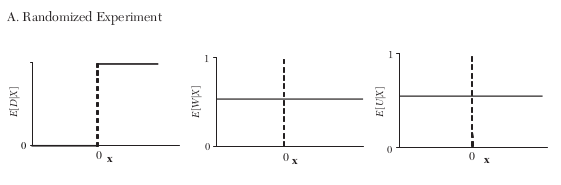
\includegraphics{material/fig-5-a}}
\end{figure}

\end{frame}
%-------------------------------------------------------------------------------
%-------------------------------------------------------------------------------
\begin{frame}

\begin{figure}[htp]\centering
\scalebox{0.70}{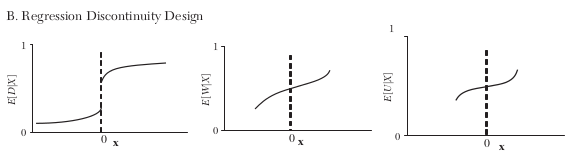
\includegraphics{material/fig-5-b}}
\end{figure}

\end{frame}%-------------------------------------------------------------------------------
%-------------------------------------------------------------------------------
\begin{frame}

\begin{figure}[htp]\centering
\scalebox{0.70}{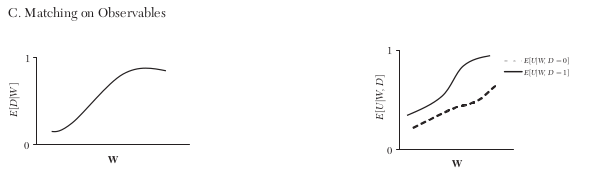
\includegraphics{material/fig-5-c}}
\end{figure}

\end{frame}
%-------------------------------------------------------------------------------
%-------------------------------------------------------------------------------
\begin{frame}

\begin{figure}[htp]\centering
\scalebox{0.70}{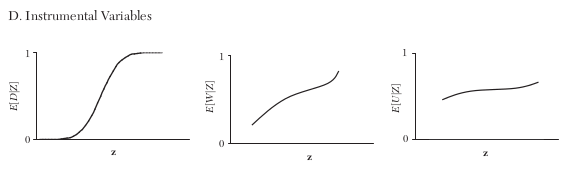
\includegraphics{material/fig-5-d}}
\end{figure}

\end{frame}
%-------------------------------------------------------------------------------
%-------------------------------------------------------------------------------
